%==============================================================================
%  GenAI4Health @ NeurIPS 2026 --- DEMONSTRATION PAPER TRACK
%
%  HARD CONSTRAINTS (from the CFP -- re-check before submitting):
%    * 5 pages max, EXCLUDING acknowledgements, references, appendix
%    * neurips_2026.sty, anonymous (double-blind), >=2 reviewers, NO rebuttal
%    * Deadline: 5 September 2026, 11:59pm AoE.  Notification: 29 September.
%    * The track wants "a functioning system -- deployed, in pilot, or a working
%      prototype" plus "evidence that the system works as described (screenshots,
%      example interactions, a video link, usage statistics, or preliminary user
%      feedback)".  QUANTITATIVE EVALUATION IS NOT REQUIRED.  Mockups are not OK.
%
%  READ THIS FIRST -- the single biggest risk is over-scoping.  You have a large
%  system and 5 pages.  The paper carries ONE argument; everything else goes to
%  the appendix or the repo.  Cut ruthlessly and cut early.
%
%  ANONYMISATION CHECKLIST (do this before you upload anywhere):
%    [ ] no author name / email / ORCID in this file
%    [ ] anonymous repo mirror; scrub `git log` (author name is in every commit)
%    [ ] .env is gitignored AND was never committed -- check history, not just HEAD
%    [ ] no institution name in figure captions, screenshots, or file paths
%    [ ] screenshots: no macOS username visible in a title bar or URL
%==============================================================================

\documentclass{article}

% THIS venue is a double-blind WORKSHOP, so the option is `dblblindworkshop`
% (not `final`, which would de-anonymise you, and not the bare package, which
% formats for the main track).  For the camera-ready in October, add `final`:
%     \usepackage[dblblindworkshop, final]{neurips_2026}
\usepackage[dblblindworkshop]{neurips_2026}
\workshoptitle{GenAI for Health}   % printed in the page footer; required by the
                                   % workshop options or the footer reads "Workshop: ."

\usepackage[utf8]{inputenc}
\usepackage[T1]{fontenc}
\usepackage{hyperref}
\usepackage{booktabs}
\usepackage{amsfonts}
\usepackage{amsmath}
\usepackage{amssymb}   % logic.tex
\usepackage{amsthm}    % logic.tex
\usepackage{stmaryrd}  % logic.tex: \llbracket \rrbracket, the denotation brackets
\usepackage{microtype}
\usepackage{graphicx}
\usepackage{xcolor}
\usepackage{listings}
\usepackage{float}

% ---------------------------------------------------------------------------
% Figures: plain \includegraphics over the pre-rendered PDFs in figures/,
% no macro indirection. Each diagram is AUTHORED as SVG (figures/*.svg, kept
% for editing) and rendered to the PDF that is actually included -- edit the
% .svg, then regenerate its .pdf:
%     python3 -c "import pymupdf as fitz; \
%       open('name.pdf','wb').write(fitz.open('name.svg').convert_to_pdf())"
% MuPDF's SVG parser ignores <style>/class rules (falls back to black fill for
% every shape), so each source SVG has its styling flattened to inline
% style="..." attributes -- already done for every file in figures/, so this
% only matters again if you edit a diagram.
% ---------------------------------------------------------------------------
\graphicspath{{figures/}}

%------------------------------------------------------------------------------
% Drafting aids.  Set \draftmodetrue while writing; flip to false to see the
% real page count.  DO NOT SUBMIT WITH NOTES VISIBLE.
%
% \note MUST be \long (its argument spans paragraphs and itemize blocks) and
% MUST use \color inside a group rather than \textcolor{}{} -- \textcolor takes
% a SHORT argument, so a blank line inside one gives:
%     "Paragraph ended before \@textcolor was complete."
% Also: never put verbatim/lstlisting inside \note{...}.  A verbatim environment
% cannot appear in a macro argument at all.  Code blocks go OUTSIDE the note,
% wrapped in \ifdraftmode ... \fi.
%------------------------------------------------------------------------------
\newif\ifdraftmode
\draftmodetrue          % <-- set to \draftmodefalse before submitting

\ifdraftmode
  \long\def\note#1{\par\begingroup\small\sffamily\color{blue!65!black}%
                   \leftskip=1em [#1]\par\endgroup\normalsize\normalcolor}
  \newcommand{\todo}[1]{{\color{red!80!black}\bfseries [TODO: #1]}}
  \newcommand{\budget}[1]{\marginpar{\scriptsize\color{gray}#1}}
  \newcommand{\num}[1]{{\color{orange!85!black}#1}}   % un-verified number
\else
  \long\def\note#1{}
  \newcommand{\todo}[1]{}
  \newcommand{\budget}[1]{}
  \newcommand{\num}[1]{#1}
\fi

% Code blocks: use \begin{cmds}...\end{cmds}, never inside a \note.
\lstnewenvironment{cmds}{\lstset{basicstyle=\ttfamily\scriptsize,frame=single,
  framesep=4pt,columns=fullflexible,breaklines=true,xleftmargin=0pt,
  aboveskip=6pt,belowskip=6pt}}{}

\lstset{basicstyle=\ttfamily\scriptsize, frame=single, framesep=4pt,
        columns=fullflexible, breaklines=true, xleftmargin=0pt}

% Required by logic.tex, which states the guards as propositions.
% NOTE: logic.tex is NOT \input yet. Two places refer to its content in prose
% rather than by \ref, so nothing dangles; if you merge it in, turn
% "the determinacy proposition" (Sec. 5) and the propositions row in the
% reproducibility table back into real \ref's.
\newtheorem{proposition}{Proposition}
\newtheorem{corollary}[proposition]{Corollary}

%==============================================================================
\title{GuidelineForge: Guideline Formalisation\\
       with Provenance, Refusal, and Three-Valued Verdicts}
% ALTERNATIVES, in case a co-author hates the above:
%   The Residue Is the Deliverable: An Auditable Pipeline from Clinical
%     Guidelines to Executable Checks
%   Don't Stub, Don't Guess: Formalising Clinical Guidelines with Named Holes
% Pick one and stop -- the title is not where your remaining hours go.

% In anonymous mode the style file IGNORES this block and prints its own
% "Anonymous Author(s)" instead -- so put the real details here now and they
% will simply appear when you add the `final` option for the camera-ready.
\author{%
  Author Name \\                    % <-- REPLACE (plain text, not \todo:
  Department \\                     %     \todo vanishes when draft mode is off,
  Institution, City, Country \\     %     which would leave this block empty in
  \texttt{name@institution.edu}     %     the camera-ready)
}

\begin{document}
\maketitle

%==============================================================================
\begin{abstract}
\note{WRITE THIS LAST. Six sentences, in this order --- the shape is doing work:
(1) LLM pipelines that turn clinical guidelines into executable logic are scored
on coverage; (2) coverage rewards the one failure that matters, because a rule
that is silently wrong looks exactly like a rule that works; (3) we demonstrate
a system whose primary output is the rule set AND a per-statement account of
everything it declined to encode, with reasons and source spans; (4) name the
three mechanisms --- retrieval-not-generation for codes, named holes instead of
stubs, deontic force as an operator; (5) say what a viewer can DO with the demo
(upload a guideline, check a patient, see the residue); (6) one honest sentence
on scope --- n documents, n rules, no clinician adjudication yet.

Do not put a specific formalizability-ceiling percentage in the abstract --
that measurement was cut from the paper as too fragile to hang a claim on
(single annotator, same model family, $n=45$); the residue's value is argued
qualitatively in Method (\S\ref{sec:design}) instead.}

Our contributions are as follows: we present a pipeline that converts an open-access guideline document into executable CQL and a three-valued checker, in which every emitted rule cites the exact source sentence it was derived from. We treat refusal as a measured output, reporting six distinct reasons a statement could not be encoded alongside the rules that were successfully produced for users to be aware of. We keep an undefined predicate as a free variable rather than substituting a default, which we show changes the verdict returned for a real patient record. Finally, we treat deontic force as an operator on the rule in the language itself rather than a label attached after the fact, so that a permission has no violating patient by construction.

\end{abstract}

%==============================================================================
\section{Introduction}
\label{sec:intro}
\budget{1.5 pp}

Clinical practice guidelines specify, in natural language, the conditions under which a given action — a drug, a test, a referral — should or should not be taken. Because that language is written for a clinician rather than a machine, guidelines are not directly checkable against a patient record: confirming that a care plan follows a recommendation still requires a person to read the sentence and reason about the case by hand. A growing body of work translates guideline text into a machine-checkable representation that can be run against structured patient data. PathWISE uses a five-stage LLM pipeline separating knowledge extraction from executable clinical logic \citep{pathwise}; Xie and Du use a SAT solver to detect logical inconsistencies between recommendations that standalone LLMs miss \citep{xiedu}; MedGuideX compiles guidelines into executable decision functions and uses them as a training oracle \citep{medguidex}; Leonardi et al. derive rules from guideline text and score conformance across an event log of patient traces \citep{leonardi}.

Systems of this kind are almost universally evaluated, and in practice optimised, for \emph{coverage}: the fraction of guideline statements successfully translated into a rule. Coverage is cheap to compute and rises monotonically as a system is made more permissive, but it cannot distinguish a rule faithful to its source from one that is not. A predicate the formaliser cannot pin down can be filled with a default and counted as encoded; two names for the same clinical concept can be treated as distinct symbols, yielding a rule that is well-formed but vacuous. Neither failure fails a syntax check, and both raise the coverage number.

This motivates the position we take: a system that reports it could not encode a statement makes a true claim about its own limits, while a system that silently produces an unfalsifiable rule makes a false claim about the patient. We argue that refusal should be a first-class, measured output rather than a failure to be minimised, and describe a system built on that principle.

Three approaches to the underlying problem each fail to prevent this class of error, for specific and demonstrable reasons. The first is \textbf{substituting a default}. Faced with a guideline stating that a drug should be started ``if eGFR is below 30 or the patient is at high risk'' without defining high risk, PathWISE substitutes \texttt{false} for nodes its audit marks uncomputable, preserving compilability while surfacing the node for human review \citep{pathwise}. Its authors describe the choice between this and emitting a partial definition as an open governance question. The question is empirical, and the substitution is not neutral: \texttt{false} in a conjunctive position removes the branch, so a patient qualifying only via that criterion is never routed down it. Section~\ref{sec:necessity} quantifies how often such a default changes a verdict.

The second is \textbf{detecting vagueness by sampling for disagreement} \citep{ksample}: a genuinely ambiguous statement admits multiple readings, so repeated formalisation attempts should disagree, yielding a signal that needs no labelled data. This assumes a model facing ambiguity guesses differently each time rather than settling on one answer — or one refusal. Nothing guarantees it. Given \textit{eGFR below 45 and the patient is frail,''} a model need not produce several guesses at frail''; in our runs it recognised the same gap on every attempt and declined consistently, leaving no disagreement to detect even though the statement is genuinely underspecified. The method fails precisely where it is needed. Our gate instead makes refusal an explicit branch of a single constrained decode, so the signal is available from one call.

The third is \textbf{asking a model directly whether a statement is too vague to formalise}. This is circular — the model that struggles with vague language adjudicates its own vagueness — and empirically weak even when purpose-built, reaching around 0.71 F1 \citep{errorcat}. 

\todo{Insert the demo URL and the video link here, anonymised.}


\note{THIS IS THE SECTION THE TRACK ACTUALLY ASKS FOR. Three scenes, each with a
screenshot. Write it as ``what a viewer sees'', not as a feature list.

\textbf{Scene 1 --- upload.} A real PMC guideline goes in; the dashboard shows
rules, refusals grouped by reason, and the awaiting-formalisation count side by
side. The point to make: a checker that shows only what compiled tells a
governance reader the tool covered everything. Shot: the dashboard grid, then
the upload modal.

\textbf{Scene 2 --- one statement, adjudicable.} The HTML report puts the source
sentence beside the rule it became, with the guideline's own wording of its
strength. Use the PMC12355350:0048 case: the sentence ends ``\ldots and a weak
recommendation against finerenone in adults with CKD'' and the rule beside it is
only about SGLT-2i/GLP-1, so the dropped clause is visible at a glance. Shot:
one statement card, cropped.

\textbf{Scene 3 --- a patient, and a verdict that is not yes/no.} Post a patient
and plan, and get MAY-violate with a minimised counterexample rendered in prose
(``it becomes a certain violation if potassium check occurred = false''). Shot:
the verdict badge and the prose counterexample.

Then record a 2--3 minute screen capture of these three scenes and link it. The CFP names video explicitly and it is the cheapest evidence you can produce.}

\todo{Take the three screenshots, put them in figures/, and lay them out as a
2- or 3-panel figure. Crop tightly --- a full browser window wastes the page.}

%==============================================================================
\section{Method}
\label{sec:design}
\budget{1.25 pp}
\subsection{Pipeline architecture}

Details of the 4 stages of the pipeline: extraction, grounding, formalization, and checking are outlined below (Figure~\ref{fig:arch}). Extraction takes a guideline document and produces a \emph{statement}: a span of text that is verbatim and locatable, carrying a locator and character offsets that let it be re-found in the source. Grounding takes a statement and produces a \emph{registry}: a closed vocabulary in which every name has been resolved to a version-pinned clinical code, or, when it could not be resolved, is declared absent rather than guessed. Formalization takes a statement and a registry and produces a \emph{rule} $\Phi_R = \mathit{when} \rightarrow \mathit{then}$ under a deontic operator, decoded against a grammar whose variable and event names are exactly the registry's to ensure an unknown name is not a decoding error to be caught after the fact, but a symbol the grammar does not contain. Checking takes a rule and a partial patient record and produces: 1) one of the three-valued verdicts of Proposition ~\ref{prop:exhaustive} (\textsc{must-violate}, \textsc{certified-compliant}, and \textsc{may-violate}), and 2) a minimized witness when the verdict is undetermined (\S\ref{sec:may}).

Only four of the pipeline's components call an LLM, and each is built so that its output space is too small to contain the pipeline's characteristic failure mode. The mention proposer returns exact substrings of the sentence under formalization, never a free-form description of a clinical concept. The terminology selector is shown a numbered list of candidate codes and returns an index into that list, or abstains; a hallucinated code is not a value the selector's output type can express. The rule decoder's variable and event enumerations are populated directly from the registry a given statement produced, so a concept that failed to bind in grounding cannot subsequently appear in a rule. Every other component -- normalization, retrieval, validation, the solver checks of Section~\ref{sec:necessity}, the lowering to CQL -- is deterministic and requires no model call. The lowering is not merely emitted: every rule the pipeline produces is compiled by HL7's own \texttt{cql-to-elm} translator before it is shipped, and a rule whose CQL the translator rejects is recorded as such rather than counted as encoded. An absent toolchain is reported as absent, never as a pass.

A statement that cannot be carried through this narrowing is not discarded: it becomes a \emph{refusal}, one of the six reason codes of Table~\ref{tab:attribution} (Appendix~\ref{app:repro}). The residue a guideline leaves behind is measured with the same rigour as the rules it yields, which is the property a coverage number alone cannot provide -- a refusal reason is itself informative about the guideline (a vague qualifier, a permissive recommendation, an obligation the source states is overridable), not merely an honest admission of the tool's limits. Two of the six reasons are set deterministically, and the remaining four are gated by deterministic checks even where the final call is the model's, rather than taken on the model's word alone.

\begin{figure}[t]
  \centering
  \includegraphics[trim=5cm 5cm 4cm 6cm, width=1\linewidth]{figures/achitecture.pdf}
    \caption{The pipeline's four stages in detail. Shaded components are the four model calls; every other component is deterministic. The channel along the bottom is the declared residue.}
  \label{fig:arch}
\end{figure}

%==============================================================================
%  SECTION 5.  This is the ELABORATE version -- longer than 5 pages can hold.
%  Cut in this order: (1) the hole-position table to the appendix, (2) the
%  per-row prose down to one sentence each, (3) the robustness paragraph.
%
%  Measured over the GENERATED rule set only.  The table over the system's own
%  19 rules was cut: every row rested on 2 to 6 rules, and it disagreed with
%  this table in magnitude for reasons we could not isolate.  The harness still
%  produces it (python3 ablation.py --plans 50 --seed 0), so it can come back
%  if the corpus grows.
%==============================================================================

\subsection{Justification for design choices}
\label{sec:necessity}
\subsubsection{Procedure}
We perform an ablation with every guard in the checker, and measure the difference in verdicts about a patient. For a rule $R$ and a partial patient record $P$ we compute the verdict of the
full system and of the system with exactly one guard disabled, and record
whether the verdict moved and in which direction. Records are drawn from the
solver, so every value satisfies the domain theory; each record pins a random
subset of the rule's variables and leaves the rest free, since a fully
determined record admits no \textsc{may-violate} and would make the comparison
vacuous. Half of each rule's records are drawn from $\mathcal{D} \wedge \neg
\Phi_R$ -- completions in which the rule really is broken -- because
uniformly sampled records almost never reach the region where two encodings
disagree. Runs are deterministic given a seed; see Appendix~\ref{app:repro}. Verdicts are \textsc{must-violate}, \textsc{certified-compliant} and \textsc{may-violate} for an obligation, and \textsc{option-taken},
\textsc{option-not-taken}, \textsc{option-available} and \textsc{option-not-applicable} for a permission. A change to verdict is counted when:
\begin{itemize}\itemsep1pt
  \item the ablated verdict is \textsc{certified-compliant} and the full
        verdict is not -- a patient cleared where the source was silent; false positive
  \item the ablated verdict is \textsc{must-violate} and the full verdict is
        not; false alert
\end{itemize}
For a rule whose full verdict is any \textsc{option-} state, \emph{any}
violation verdict counts as the second case, \textsc{may-violate} included: the
permission lattice has no accusing state, so reporting that a patient may have
deviated is already the harm. Transitions within a lattice
(\textsc{option-available} to \textsc{option-not-taken}) and losses of
certainty in the safe direction (\textsc{must-violate} to
\textsc{may-violate}) are recorded but not counted in either column.

The rules are generated. Measured over the rules the system happens to have produced, each row would rest on between $2$ and $6$ rules -- not a sample but an accident of which guidelines are open access. We therefore enumerate the space the language can express: undefined predicate in the antecedent, in the consequent, or absent; obligation or permission; numeric threshold, boolean, time window, or relative change; one atom, two under conjunction, or two under disjunction. Two instances per cell over $72$ cells gives $144$ rules. Every generated rule is put through the same \texttt{validate\_rule} function and non-degeneracy check the pipeline applies to a rule a model wrote, and no candidate was rejected -- so each is a rule the system would have accepted.

\subsubsection{Results}

\begin{table}[t]
  \centering
  \caption{$144$ rules, up to $50$ records each (mean $40.0$; a rule
  with few variables admits fewer distinct partial records), $5{,}760$ rule-record pairs. \emph{Applies to} counts the pairs the guard can act on at all -- a substitution needs a boolean undefined predicate, the deontic row a permission, the occurrence row a time window --- and both percentages are over those. Zero means the guard never moves a verdict that way.}
  \label{tab:generated}
  \begin{tabular}{lrrr}
    \toprule
    & & \multicolumn{2}{c}{verdict moved to} \\
    \cmidrule(l){3-4}
    Guard removed & applies to & \textsc{certified-compliant} & \textsc{must-violate} \\
    \midrule
    Undefined predicate $\rightarrow$ \textsf{false} & 4304 & 207 (4.8\%) & 170 (4.0\%) \\
    Undefined predicate $\rightarrow$ \textsf{true} & 4304 & 115 (2.7\%) & 219 (5.1\%) \\
    Deontic operator (all rules obligations) & 2876 & 0 (0.0\%) & 2300 (80.0\%) \\
    Occurrence flag on a time window & 1713 & 120 (7.0\%) & 0 (0.0\%) \\
    Three-valued verdict $\rightarrow$ single query & 5760 & 0 (0.0\%) & 1776 (30.8\%) \\
    \bottomrule
  \end{tabular}
\end{table}

Row 1 is PathWISE's stated default --- stubbing uncomputable nodes as
\textsf{false} to preserve compilability \citep{pathwise}. Every guideline in
the corpus states predicates it never defines, and substituting a value for
one is unsafe in both directions, by position:
\textsf{false} in the \emph{antecedent} narrows applicability and clears
patients, while the same substitution in the \emph{consequent} makes the
obligation unsatisfiable and manufactures alerts, broken down by position in
Table~\ref{tab:holepos} (Appendix~\ref{app:extra}). Both columns above
average over that split, since half the generated rules are permissive; restricted to
obligations, substituting \textsf{false} clears $9.6\%$ of pairs and accuses
$7.9\%$, and substituting \textsf{true} accuses $10.2\%$ and clears $5.3\%$ ---
the same magnitudes with the directions exchanged. The largest effect
measured is dropping the deontic operator: once a rule is permissive, this
changes the verdict for four pairs in five, always into an alert on a patient
who declined an option the source offered. Dropping the occurrence flag on a
time window lets a patient who was never tested satisfy the window, because
the solver selects a small day count; all $120$ divergences move to
compliant, and the rate is low only because the flag is decisive exclusively
when the rest of the record already leaves the window in question, not
because it rarely matters when it applies. The three-valued verdict is the
only row whose correctness is a theorem rather than an argument: a single
satisfiability call returns the same answer for ``every completion violates''
and ``some completion violates'', so it reports both as violations; measured
against $\neg\Phi_R$ instead of the rule's own violation condition the figure
reads $71.1\%$, which double-counts the deontic row above it.

Note that the generated vocabulary assigns every numeric variable a plausible physiological range; the pipeline currently supplies none, so a rule it produces is checked against a weaker domain theory. Re-running the sweep with the ranges stripped ($5{,}800$ pairs rather than $5{,}760$, since the sampler explores a wider space) moves every rate by less than half a point --- substituting \textsf{false} clears $4.8\%$ of applicable pairs with the ranges and $4.9\%$ without, and the single-query row reads $30.8\%$ against $30.6\%$ --- so the result does not rest on that difference.

\subsubsection{Justification for undetermined verdicts}
\label{sec:may}

A verdict of \textsc{may-violate} is only useful if the reader is told what it
turns on. \texttt{minimal\_counterexample\_core} returns the smallest set of those values that on its own forces the violation, by deletion-based extraction: drop one assignment, keep the drop if the remainder still cannot be made compliant. Because the check leaves every non-core variable unconstrained, unsatisfiability quantifies over all their completions, so the core's values force a violation \emph{whatever the unmeasured variables turn out to be}. The result is minimal, not minimum: an irreducible set, not provably the smallest, so sizes are an upper bound.

\begin{center}
\begin{tabular}{rrrrr}
  \toprule
  unstated variables & verdicts & mean core & reduction & single-variable core \\
  \midrule
  1 & 396 & 1.00 & 1.00$\times$ & 100.0\% \\
  2 & 619 & 1.29 & 1.56$\times$ & 71.4\% \\
  3 & 479 & 1.58 & 1.90$\times$ & 50.1\% \\
  4 & 205 & 1.78 & 2.25$\times$ & 34.6\% \\
  5 &  76 & 1.97 & 2.53$\times$ & 21.1\% \\
  6 &   8 & 2.50 & 2.40$\times$ & 0.0\% \\
  \bottomrule
\end{tabular}
\end{center}

Of $5{,}764$ records, $1{,}783$ returned \textsc{may-violate}. The core is smaller than the set of unstated variables ($1.39$ against $2.42$ on average), and the reduction grows as the record thins, because the core is bounded by the rule's structure -- the number of atoms that must be forced -- and not by how much the record omits.


$1{,}165$ of the $1{,}783$ undetermined verdicts ($65.3\%$) rest on a single variable, but $126$ of those name an \emph{undefined predicate} -- a phrase a
source states and never defines -- which no measurement resolves, because there is nothing to measure. Splitting them: $1{,}039$ ($58.3\%$) turn on a single bound concept, $126$ ($7.1\%$) on a single undefined predicate, and across all
core sizes $251$ ($14.1\%$) involve an undefined predicate somewhere. A system that substituted a value for those predicates would return a definite verdict in every one of those cases, and would be asserting something the source does not say each time. Therefore, the distinction is \emph{visible} -- the system can say which undetermined verdicts are waiting on a measurement and which are waiting on a definition the source never gave.

That a core is a single variable does not mean measuring it answers the
question: the core is sufficient for \emph{one} outcome, those values force a
violation, but a different value of the same variable may leave the verdict
open. The claim a clinical reader takes from ``measure $X$'' is stronger --
that \emph{every} value of $X$ determines the verdict -- and whether it holds
is decidable without enumerating values (Proposition~\ref{prop:settle}).

Of the $1{,}183$ single-variable cores this experiment sees, measuring the named
variable determines the verdict in $840$ ($71.0\%$), which is $46.6\%$ of all
undetermined verdicts. In the other $343$ ($29.0\%$) some value of it leaves the
case open, and $147$ of those name an undefined predicate, where no measurement
exists to take. The naive reading --- counting single-variable cores as
resolvable measurements --- would have claimed $65.7\%$ and overstated by nearly
a third. (This experiment and the core-size table above are two draws from one
sampler rather than two views of one sample, so their \textsc{may-violate}
counts differ slightly; see Appendix~\ref{app:repro}.)

\subsection{Language design}

\begin{figure}[H]
    \centering
    \includegraphics[trim=0cm 11cm 0cm 0cm, clip, width=\linewidth]{figures/language_shorten.pdf}
    \caption{The rule language, with one worked example at every layer.}
    \label{fig:language_shorten}
\end{figure}

Every concept the language can talk about has to be declared and bound to a real code before it can be referenced anywhere, ensuring a term can mean exactly one thing. Conditions are built from a deliberately small grammar: four leaf comparisons (equality, range, time-since-event, change-from-baseline) and three logical connectives (negation, conjunction, and disjunction). Keeping the connective set minimal, rather than adding derived operators for convenience, means every expression reduces to a normal form, and its logical difficulty can be classified consistently, from simple propositional checks up to the temporal reasoning that "since" clauses require.

The rule itself never carries a labelled action, only a formula wrapped in an obligation or permission. The recommended action, its target, and the source sentence exist as metadata for a human reviewer, not for evaluation logic to branch on. Because not every guideline sentence can be safely reduced to this form, refusal is built-in as a legitimate output in its own right: the system is designed to say it can't encode something, rather than force a best guess. A three-valued verdict sits naturally in the target language: CQL's Boolean type is nullable, so a comparison over an element the record does not contain evaluates to \texttt{null} rather than \texttt{false}. \texttt{null} propagates through the connectives under Kleene semantics, so the unknown reaches the top-level \texttt{define} instead of collapsing at the leaf.




%==============================================================================
\section{Limitations, and what a reviewer can run}
\label{sec:limits}
\budget{0.25 pp --- flat, no hedging}

The corpus is nine open-access guidelines, and the sampling frame is not incidental: PubMed Central's open-access subset over-represents journals that publish structured, GRADE-style \citep{grade} recommendation abstracts, which are easier to segment than a guideline leaving its recommendations in narrative prose. The documents a deployment would most want — NICE, KDIGO, ACC/AHA — are not open access, so they are absent by construction. More generally, guidelines follow no common structure, which makes a representative sample hard to assemble for any system of this kind. Because the pipeline takes a document rather than a corpus, extending it is a licensing question rather than an engineering one: an institution can run it over the guidelines it has already licensed, and we would expect the residue to grow on documents whose recommendations are narrative rather than structured.

There is no reference corpus with ground truth for this task, and that is a property of the field's existing artefacts. AHRQ's CDS Connect \citep{cdsconnect} is close — it publishes decision-support artefacts — but not a labelled set of guideline sentences paired with the rules they should become. An electronic Clinical Quality Measure \citep{cql} is a cohort definition over a population, not a per-patient recommendation with a source sentence to be faithful to. A system whose contribution is the distinction between encoding a statement and declining it therefore has nothing external to be scored against. Building that corpus — sentences paired with both their intended rule and, where none exists, the reason — is the obvious next step, and the per-statement refusal log this system emits is a candidate starting point for one.
Finally, no clinician has yet adjudicated the system's output. Clinical review of the generated rules, and of the criteria by which a rule is judged faithful to its source, remains future work. The scope here is narrower by design: whether the artefact says what the sentence said, not whether the sentence should be followed.
%==============================================================================
% neurips_2026 loads natbib, so use a natbib-aware style.
\bibliographystyle{plainnat}
\bibliography{refs}
\note{refs.bib needs: PathWISE (the false-stub baseline); the K-sample /
disagreement method; the $\sim$0.71 F1 error-categorisation result; the
self-correction-is-unreliable result that justifies the bounded repair loop;
HL7 CQL; GRADE; and one or two guideline-formalisation surveys.
BE PRECISE ABOUT THE BASELINE: you did not run PathWISE. You reimplemented its
stubbing rule. Say so in one clause --- a reviewer who knows the paper will
check, and the honest phrasing costs you nothing.}

%==============================================================================
\appendix
\section{Additional results and figures}
\label{app:extra}

\note{Still to add here: the full residue log, per-document statement counts,
and the DSL grammar. The hole-position split and the two benchmarks below are
done, and their numbers come from the commands in Appendix~\ref{app:repro}.}

\paragraph{Detection: does the checker flag what it should?}
The ablation of Section~\ref{sec:necessity} shows that each guard moves
verdicts; it does not show that the verdicts are right. For that a record needs
a label fixed independently of the checker. \texttt{synthesize\_boundary\_tests.py}
supplies one: for every numeric and temporal boundary in the hand-authored
fixture rules it solves against $\Phi_R$ for a record on the compliant side and
against $\neg\Phi_R$ for one on the violating side, so each record's true label
follows from its construction rather than from our reading of the sentence.
\texttt{detection\_benchmark.py} then pins every variable and re-derives the
verdict through the ordinary checker. All $24$ boundary records matched the
label they were built to carry --- $14$ \textsc{certified-compliant} and $10$
\textsc{must-violate}, with no case flagged in the wrong direction and none
left undetermined once fully pinned. This is a small set over eight fixture
rules, not the generated sweep, so it bounds nothing about what the pipeline
emits; what it establishes is that the three-valued classifier agrees with
ground truth wherever ground truth exists.

\paragraph{What a single call reports instead, and what the second one costs.}
A three-valued verdict needs two satisfiability queries where a naive check
makes one. Over $200$ synthetic patients against $25$ bounded-horizon clauses
--- $5{,}000$ rule--patient pairs over generic \texttt{drug\_N}/\texttt{lab\_N}
names rather than the fixtures, each plan pinning $14$ of $30$ candidate
actions --- the naive single call reports a violation for $2{,}010$ pairs
($40.2\%$). The three-valued checker returns \textsc{must-violate} for none of
them: every one is a case in which some completion of the unmeasured facts is
compliant, and the naive check cannot separate that from a violation because
one query cannot distinguish ``every completion violates'' from ``some
completion violates''. These are randomly generated plans, so no certain
violation is expected --- the point is not that the naive check is wrong about
a patient but that it has no vocabulary in which to be undetermined. The
second query costs $2.1\times$ the first (Table~\ref{tab:perf}); the median
check is $25.2$\,ms and the full sweep runs in $137$\,s, so on this workload
not guessing is not what makes a check slow.

\begin{table}[h]
  \centering
  \caption{Solve time per rule--patient pair, $5{,}000$ pairs, single process,
  environment of Appendix~\ref{app:repro}. The three-valued column includes
  extracting a minimal counterexample core for every undetermined verdict
  ($2{,}010$ of them, mean core $3.27$ variables).}
  \label{tab:perf}
  \begin{tabular}{lrrrr}
    \toprule
    Check & mean & median & p95 & max \\
    \midrule
    naive, one query      & 13.0\,ms & 11.5\,ms & 20.3\,ms & 145.6\,ms \\
    three-valued, two queries & 27.5\,ms & 25.2\,ms & 42.3\,ms & 386.4\,ms \\
    \bottomrule
  \end{tabular}
\end{table}

\paragraph{Hole position.}
Table~\ref{tab:holepos} splits the two substitution rows of
Table~\ref{tab:generated} by where the undefined predicate sits, which is
what Section~\ref{sec:necessity} draws on to say the two substitutions are
unsafe in opposite directions rather than simply averaging out. The split is
exactly symmetric, and each of the four cells is empty in the direction the
argument says it should be: \textsf{false} in the antecedent only ever clears
a patient and \textsf{true} in the antecedent only ever accuses one, while in
the consequent the two exchange roles. Each substitution also has a control on
the rules with no undefined predicate at all --- nothing is substituted, and
nothing moves.

\begin{table}[h]
  \centering
  \caption{Split by where the undefined predicate sits. Each substitution has a control test: nothing is substituted and nothing moves.}
  \label{tab:holepos}
  \begin{tabular}{llrrr}
    \toprule
    Substitution & Predicate sits in & pairs & $\rightarrow$ \textsc{certified} & $\rightarrow$ \textsc{must-violate} \\
    \midrule
    \textsf{false} & the antecedent & 2152 & 9.6\% & 0.0\% \\
    \textsf{false} & the consequent & 2152 & 0.0\% & 7.9\% \\
    \textsf{false} & --- (control) & 1456 & 0.0\% & 0.0\% \\
    \addlinespace
    \textsf{true} & the antecedent & 2152 & 0.0\% & 10.2\% \\
    \textsf{true} & the consequent & 2152 & 5.3\% & 0.0\% \\
    \textsf{true} & --- (control) & 1456 & 0.0\% & 0.0\% \\
    \bottomrule
  \end{tabular}
\end{table}

\begin{figure}[h]
  \centering
  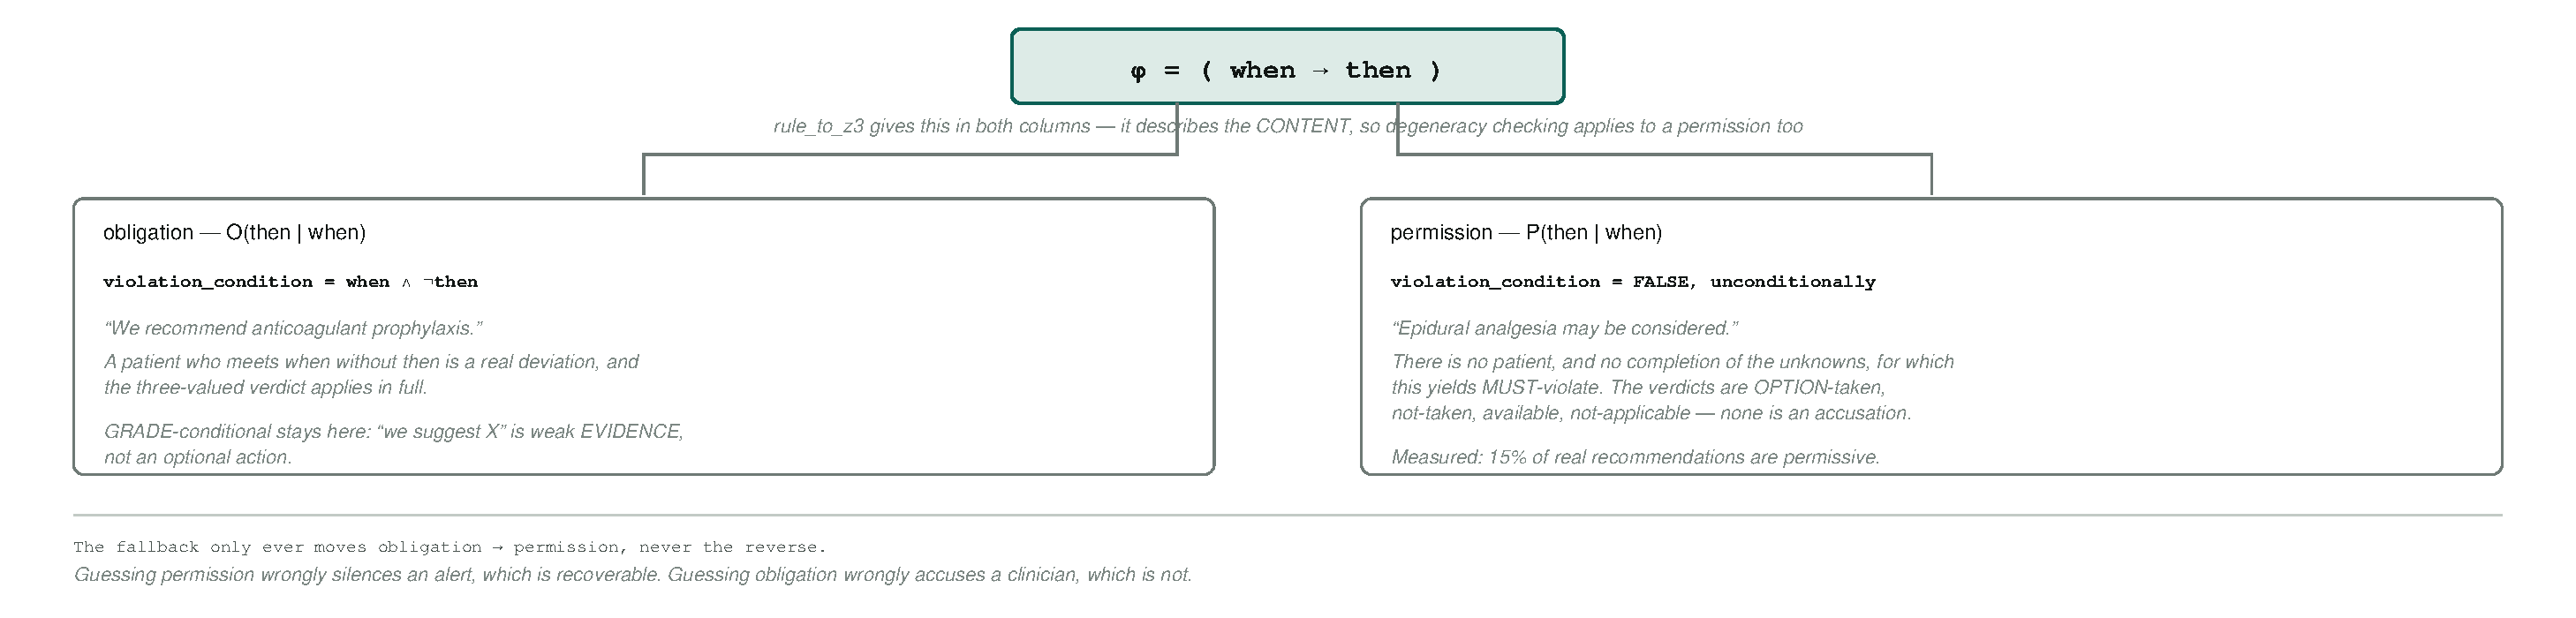
\includegraphics[width=\linewidth]{deontic.pdf}
  \caption{Obligation and permission differ in exactly one place. The violation condition of a permission is the constant \textsc{false}, so no patient and no
  completion of the unknowns can yield a violation --- a structural guarantee (Proposition 7) rather than a guard on a verdict string.}
  \label{fig:deontic}
\end{figure}

\begin{figure}[h]
  \centering
  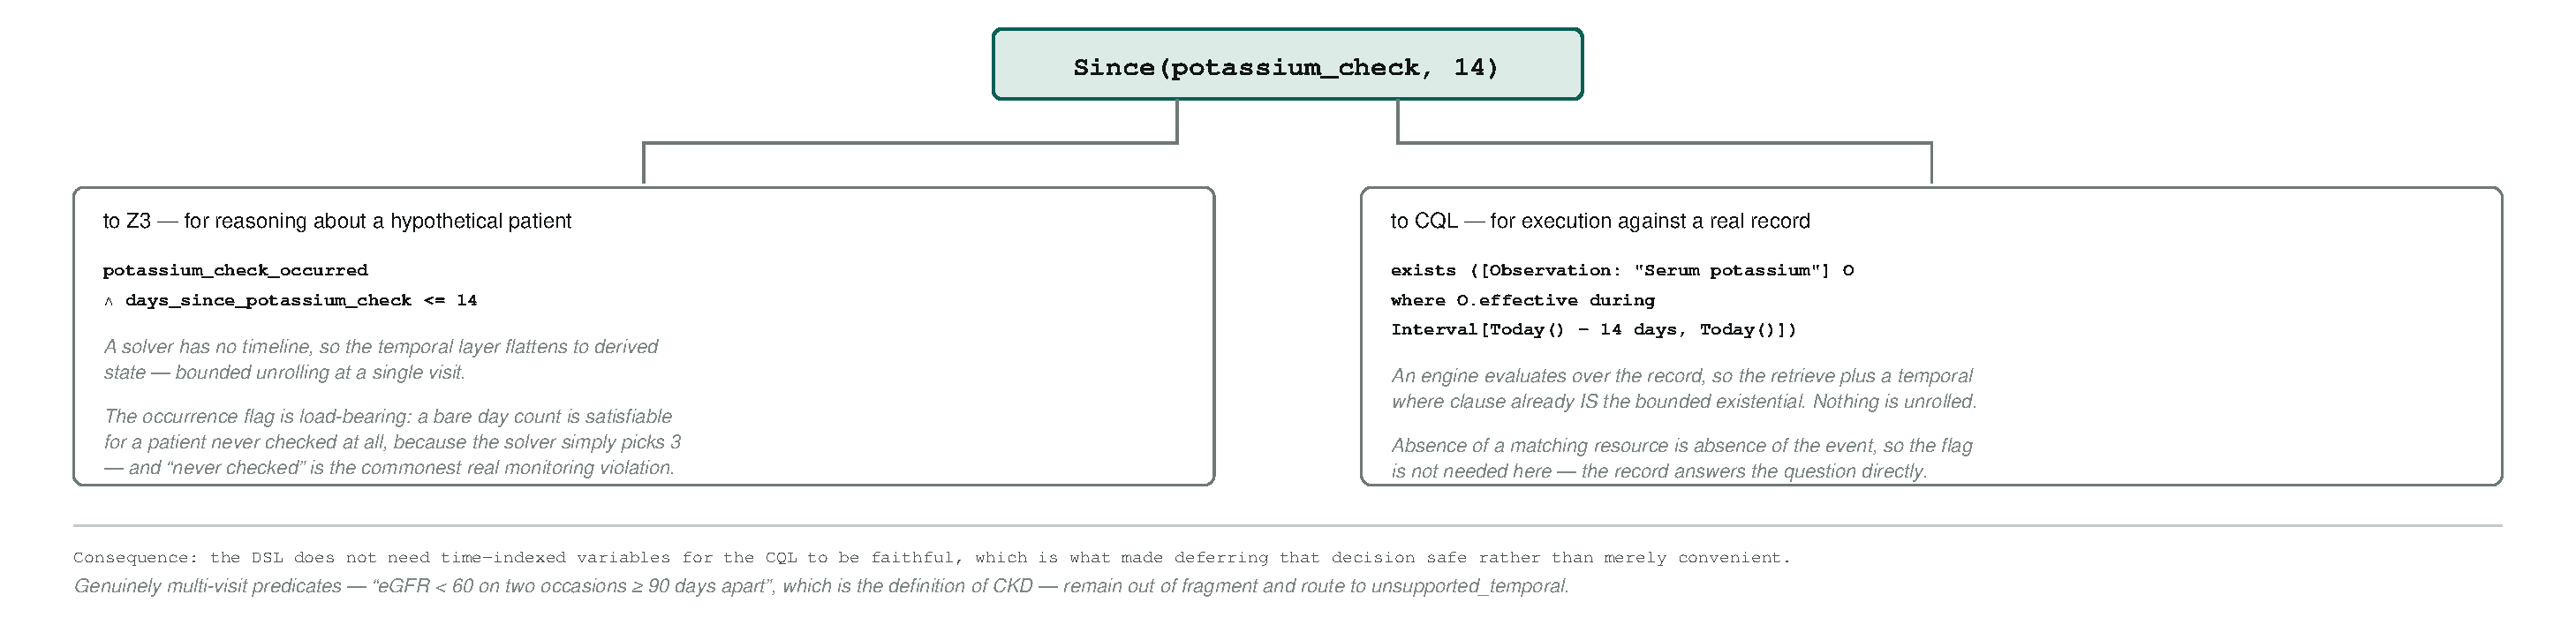
\includegraphics[width=\linewidth]{lowering.pdf}
  \caption{One node, two lowerings. A solver has no patient timeline, so recency
  flattens to an occurrence flag and a day count; a CQL engine evaluates over the
  record, where a retrieve plus a temporal \texttt{where} already is the bounded
  existential.}
  \label{fig:lowering}
\end{figure}

\section{Reproducing the measurements}
\label{app:repro}

\paragraph{Commands.}
Every number in Section~\ref{sec:necessity} and Appendix~\ref{app:extra} comes
from one of the five measurement scripts below, all in
\texttt{patient\_checker/tests}; the last two rows produce no number, and are
listed because they are what a reader would want to run next --- one prints the
rule set, the other machine-checks the propositions. None makes a model call;
none needs an API key; each is invoked separately, for the reason given under
\emph{Determinism} below.
\begin{center}
\begin{tabular}{ll}
  \toprule
  Produces & Command \\
  \midrule
  Tables \ref{tab:generated}, \ref{tab:holepos}
    & \texttt{ablation.py -{}-generated -{}-plans 50 -{}-seed 0} \\
  Core sizes, \S\ref{sec:may}
    & \texttt{explanation\_size.py -{}-plans 50 -{}-seed 0} \\
  Both \textsc{may} experiments, \S\ref{sec:may}
    & \texttt{may\_actionability.py -{}-plans 50 -{}-seed 0} \\
  Detection against ground truth, App.~\ref{app:extra}
    & \texttt{detection\_benchmark.py} \\
  Table \ref{tab:perf}, and the naive check's rate
    & \texttt{benchmark.py} \\
  The rule set itself
    & \texttt{generated\_rules.py -{}-list} \\
  \addlinespace
  The propositions stated in \texttt{logic.tex}
    & \texttt{propositions.py} \\
  \bottomrule
\end{tabular}
\end{center}
Each writes a CSV of per-verdict rows beside a short summary, both in the
artefact; the summaries are what the tables quote.
\texttt{detection\_benchmark.py} imports \texttt{synthesize\_boundary\_tests.py}
and re-solves its boundary records rather than reading a stored file, so the
labels it checks against are regenerated on every run and cannot drift from the
rules. Three variants are runnable and not reported: \texttt{ablation.py}
without \texttt{-{}-generated} runs over the rules the pipeline itself
produced, \texttt{-{}-no-ranges} strips the plausible ranges from the generated
vocabulary, and \texttt{differential\_check.py} evaluates a second,
independently worded encoding of three fixtures against the same boundary
records --- a hand-built stand-in for a dual-encoding pass, too small to report
as a result.

\paragraph{Environment.}
Python 3.14.2, \texttt{z3-solver} 5.1.0, macOS 15.5 (arm64). The commit is
recorded in the artefact. Beyond the standard library these scripts need only
\texttt{z3-solver} and the repository's own modules --- three of them reach the
checker through \texttt{api.py}, which pulls Flask in with it, though no server
is started and no port is opened. The timings in Table~\ref{tab:perf} are from
this machine, single process, with no other load.

\paragraph{Determinism.}
Runs are reproducible byte for byte given the seed: three separate processes
produce identical CSVs. This required one fix worth recording, because it is
the kind of thing that silently invalidates a reported number. A rule's
variable map is built from a Python \emph{set}, whose iteration order varies
between processes under hash randomisation; the record sampler drew from that
order, so the same seed gave different counts run to run (for one row, $103$
against $104$). The sampler now sorts the names. Anyone reproducing a
solver-driven measurement in Python should check this specifically --- the
symptom is a stable seed with unstable output, and it is invisible within a
single process.

A second limit bounds that guarantee. Each script is reproducible \emph{in its
own process}, but calling the record sampler twice inside one process is not:
at seed $0$ the first pass draws $5{,}764$ records and the second $5{,}760$,
which is exactly the gap between the record counts \texttt{explanation\_size.py}
and \texttt{ablation.py} report. The cause is below our code --- Z3 carries global state
that constructing a fresh solver does not reset, so the second pass draws
different models. Two consequences. Each script must be
invoked separately, which is how the commands above are written. And two scripts
at the same seed do not see an identical record set, so figures from
\texttt{ablation.py} and \texttt{may\_actionability.py} are two samples from one
sampler rather than two views of one sample, and are not row-for-row comparable.

\paragraph{Record counts.}
\texttt{-{}-plans} is a \emph{ceiling}, not a quantity. A record pins a subset
of a rule's variables, so a rule with few variables admits few distinct
records: at \texttt{-{}-plans 50} the actual counts range from $5$ to $50$
(mean $40.0$ over $144$ rules, $5{,}760$ pairs), and the distribution is
bimodal --- $100$ rules reach the ceiling while $8$ admit only $5$ records
each. The unit of analysis is therefore the rule--record pair, and rules
contribute unequally: a reported rate is not the fraction of \emph{rules}
affected.

\paragraph{How \emph{applicable} is determined.}
Every rate is over the pairs the guard can act on, and that set is defined in
code (\texttt{ablation.applies}) rather than by a convention in this paper, so
it is reproducible and auditable:
\begin{center}
\begin{tabular}{ll}
  \toprule
  Guard & Applies to a rule when \\
  \midrule
  substitute \textsf{false} / \textsf{true}
    & it has an undefined predicate of \emph{boolean} sort \\
  deontic operator
    & it is a permission \\
  occurrence flag
    & it mentions an occurrence flag, i.e.\ it contains a time window \\
  three-valued verdict
    & always \\
  \bottomrule
\end{tabular}
\end{center}
The boolean restriction matters: an unbound \emph{event} also leaves free
symbols behind, but they are integer and real valued, and substituting a truth
value into a quantity is meaningless. Those rules are excluded from the
substitution rows rather than coerced. Reporting over all pairs instead would
dilute every rate by the rules the guard cannot touch --- on the generated set
that is $1{,}456$ of $5{,}760$ pairs for the substitution rows alone, and
$4{,}047$ for the occurrence-flag row, which applies to only the $1{,}713$
pairs whose rule contains a time window.

\paragraph{Artefacts.}
\texttt{ablation.py} writes one row per (rule, record, guard) with columns
\texttt{source}, \texttt{rule\_id}, \texttt{deontic}, \texttt{holes},
\texttt{pinned}, \texttt{ablation}, \texttt{applies}, \texttt{full},
\texttt{ablated}, \texttt{direction} --- $28{,}800$ rows, one per
(rule, record, guard) over five guards.
\texttt{explanation\_size.py} writes one row per undetermined verdict with the
count of unstated variables, the core size, and the core's variable names.
\texttt{may\_actionability.py} adds, per verdict, the verdict after the core is
supplied and whether measuring a single-variable core determines the outcome.
Every table in Section~\ref{sec:necessity} can be recomputed from these rows
independently of the scripts' own counters, which is how they were checked.

\paragraph{Verdict transitions.}
The two columns of Section~\ref{sec:necessity} record only whether a verdict
became \textsc{certified-compliant} or \textsc{must-violate}. The full
transition matrix is recoverable from the artefact and is worth inspecting:
printing it is what exposed three separate confounds in the harness, in each
case an ablation that was changing more than one thing at once. Two examples
that are recorded but counted in neither column: a move within the permission
lattice (\textsc{option-available} to \textsc{option-not-taken}), and
\textsc{must-violate} degrading to \textsc{may-violate}, which loses certainty
in the safe direction.

\paragraph{Replaying the pipeline itself.}
The measurements above concern the checker and need no model. The extraction
pipeline does call one, and a recorded run is replayed offline by
\texttt{python3 -m pytest test\_replay.py}: prompts are stored as SHA-256
hashes with their responses, so the pipeline can be re-executed without an API
key and without redistributing source documents. A tape that no longer matches
the code \emph{skips} rather than passes.

\paragraph{Refusal attribution.}
Table~\ref{tab:attribution} backs the claim in Section~\ref{sec:design} that
refusal is not simply taken on the model's word: it is verified against the
assignment sites in the gate, and pinned by \texttt{test\_gate.py}, which
fails if any deterministic path starts assigning \texttt{unsupported\_temporal}.

\begin{table}[h]
  \centering
  \caption{Who decides each refusal. Verified against the assignment sites, and
  pinned by \texttt{test\_gate.py}, which fails if any deterministic path starts
  assigning \texttt{unsupported\_temporal}.}
  \label{tab:attribution}
  \begin{tabular}{lll}
    \toprule
    Reason code & Decided by & What sets it \\
    \midrule
    \texttt{unbound\_concept}      & deterministic & the binder: selector abstains, or no candidate \\
    \texttt{defeasible}            & deterministic & the validator: \texttt{MODAL\_PREDICATE} \\
    \texttt{beyond\_dsl}           & mixed         & \texttt{VACUOUS\_RULE}, else the model or fallback \\
    \texttt{not\_patient\_level}   & model         & the segmenter's classifier, upstream \\
    \texttt{vague\_predicate}      & model         & the formalizer declines \\
    \texttt{unsupported\_temporal} & model         & the formalizer declines \\
    \bottomrule
  \end{tabular}
\end{table}
 
\section{Engineering log}

\paragraph{Engineering log.} 
\texttt{CQL\_converter/RESULTS.md} in the anonymised repository records the full engineering log behind this pipeline: 36 dated entries, each a defect found by running real documents, with its fix and what changed as a result. It is cited here rather than reproduced -- compressing thirty-six entries into an appendix would either drown the table below or gut the entries into unverifiable one-liners. What is worth extracting is the shape common to the back half of the log: a recurring class of defect, and the structural check now in the codebase that catches every future instance of it, not only the one instance that was originally found by hand. 

\begin{table}[h]
\centering
\caption{Defect class and the structural check that now catches it, cited against \texttt{CQL\_converter/RESULTS.md} entry numbers.}
\label{tab:defect-classes}
\footnotesize
\renewcommand{\arraystretch}{1.05}
\setlength{\aboverulesep}{0.3ex}
\setlength{\belowrulesep}{0.3ex}
\begin{tabular}{p{0.32\textwidth} p{0.53\textwidth} p{0.09\textwidth}}
\toprule
\textbf{Defect class} & \textbf{Structural check now in place} & \textbf{Log} \\
\midrule
A rule compiles clean but is logically vacuous or tautological & Non-degeneracy check re-applied on every load, not only at write time --- an artefact that shipped clean can still fail on read & R14, R16, R17a \\
\midrule
A new DSL node is added; some walker's dispatch does not name it and silently treats it as absent & \texttt{test\_exhaustive.py} reads the source, enumerates every dispatch over the expression union, and fails if one omits a variant without a written reason & R34, R34a, R34c \\
\midrule
Python's \texttt{bool} is an \texttt{int}, and any non-empty string is truthy, so type-confused code silently misreads a boolean & \texttt{dsl.\_is\_number} is a codebase rule, not a one-off fix --- \texttt{bool} is never treated as a number, strings are parsed explicitly & R33b, R33c \\
\midrule
An infrastructure failure (compiler crash, auth error, empty terminology fetch) returns a value indistinguishable from a genuine negative result & Failures are labelled explicitly: a non-zero exit and a clean exit with nothing written both now raise; ``inconclusive'' is reported separately from a real disagreement & R33a, R33d, R34b \\
\midrule
A permission is encoded with the same operator as an obligation, so ``may'' reads as ``must'' & Deontic force is a dedicated operator on the rule, not a flag on a shared one, so the two cannot be conflated at decode time & R17b, R18 \\
\midrule
The partial encoding path silently drops validator evidence that the strict path keeps & Both paths now record identical validator evidence; the same discrepancy had been independently rediscovered three times before this fix stuck & R28a, R34 \\
\bottomrule
\end{tabular}
\end{table}


\note{One paragraph pointing at \texttt{CQL\_converter/RESULTS.md} in the anonymised
repo. Do NOT try to compress 36 log entries into the appendix --- cite it as an
artefact. But DO extract one table: ``defect class $\rightarrow$ the structural
check that now catches it'', with 5--6 rows. That table is the strongest thing in
the log, because it shows you can enumerate the failure classes precisely
BECAUSE you built detectors for them. Presented as a closed arc it reads as
rigour; presented as a list of past bugs it reads as a confession.}

% The logical content: what the checker's guards mean, stated as propositions.
%
% REQUIRED PREAMBLE (declare in main.tex if not already present):
%   \usepackage{amsmath, amssymb, amsthm}
%   \newtheorem{proposition}{Proposition}
%   \newtheorem{corollary}[proposition]{Corollary}
%
% Every proposition below was machine-checked against z3 before being written;
% the script is in the artefact. Proofs are short by design -- the content is
% that these are the properties the system's guards exist to preserve, not that
% any one of them is difficult.

\section{Formalisation \& logic}
\label{sec:logic}

The rule language is quantifier-free first-order logic over linear arithmetic:
propositional connectives whose atoms are arithmetic comparisons on the reals
and integers, rather than bare propositions. It is the SMT fragment
$\mathrm{QF\_LIRA}$, and is decidable. Two constructs are added --- a bounded
past-time temporal operator, flattened to derived state, and a relative-change
operator over a value at an earlier event --- and two things are deliberately
absent: quantifiers, and arithmetic relating two variables.

No rule contains a quantifier; every variable is free, which is what allows a
satisfying assignment to \emph{be} a patient. The quantification sits one level
up, in the verdict: a patient record is a \emph{partial} interpretation, and the
two definite verdicts are universal statements over the interpretations
extending it --- every completion violates, or none does --- each discharged as a
single unsatisfiability check. That is the whole reason a third verdict is
needed (Propositions~\ref{prop:determinacy} and~\ref{prop:onequery}).

Deontic force is a dyadic annotation selecting a rule's violation condition, not
a modal operator over formulas; it is never nested, which keeps the standard
deontic paradoxes out of scope. Each proposition below was machine-checked
before being stated.

\paragraph{Setup.}
A rule $R$ denotes the material implication
$\Phi_R = \llbracket \mathit{when} \rrbracket \rightarrow
          \llbracket \mathit{then} \rrbracket$
over a signature of typed variables.

\paragraph{Derived symbols.}
Two constructs are interpreted over symbols the
signature induces rather than ones a rule names directly. For each declared
clinical event $e$: $\mathsf{occ}_e$, a boolean recording that $e$ \textbf{occ}urred, and
$\mathsf{dse}_e$, an integer counting days since it did (\textbf{d}ays \textbf{s}ince \textbf{e}vent). For each event $e$ and
numeric variable $v$: $v@e$, the value $v$ held at the time of $e$. A recency
window ``$e$ within the last $n$ days'' lowers to
$\mathsf{occ}_e \wedge \mathsf{dse}_e \le n$, and a relative change ``reduce $v$
by $p$'' to $v \le (1-p)\cdot v@e$. These symbols are produced by the lowering
and never written by the generator, so each has exactly one definition.

\paragraph{The domain theory.}
The domain, $\mathcal{D}$, collects plausible physiological ranges for bound
numeric variables, code membership for coded ones, $0 \le \mathsf{dse}_e \le H$
for a fixed horizon $H$ (ten years in the implementation), and $v@e > 0$ for
each induced baseline. Unbound symbols are deliberately unconstrained --- an
axiom about a predicate the source never defined would be a claim the source
does not make. A patient record is a \emph{partial} assignment $P$: it pins the values the
record supplies and leaves every other symbol free, either because nothing
measured it or because it is an undefined predicate no data source can supply.
A \emph{completion} of the record is a model of $\mathcal{D} \wedge P$ --- one
consistent way of filling in everything the record left open. A record therefore
does not describe one patient but the set of patients compatible with it, and
the three verdicts below are statements about that whole set: every completion
violates, none does, or the record does not settle the question.
$\mathrm{Vars}(\Phi)$ denotes the symbols occurring in $\Phi$.

\[
\mathrm{verdict}(R,P) =
\begin{cases}
  \textsc{must-violate}       & \mathcal{D} \wedge P \wedge \Phi_R \ \text{unsat} \\
  \textsc{certified-compliant}& \mathcal{D} \wedge P \wedge \neg\Phi_R \ \text{unsat} \\
  \textsc{may-violate}        & \text{otherwise.}
\end{cases}
\]

\begin{proposition}[Well-posedness]
\label{prop:exhaustive}
If $\mathcal{D} \wedge P$ is satisfiable, the three above cases are mutually exclusive
and exhaustive.
\end{proposition}
\begin{proof}
Exhaustive by construction. If the first two both held, $\mathcal{D} \wedge P$
would entail both $\Phi_R$ and $\neg\Phi_R$, contradicting satisfiability.
\end{proof}

\subsection{Indeterminacy is a property of the record, not of the rule}

\begin{proposition}[Determinacy]
\label{prop:determinacy}
If $P$ assigns every symbol of $\mathrm{Vars}(\Phi_R)$ and $\mathcal{D} \wedge P$
is satisfiable, then $\mathrm{verdict}(R,P) \neq \textsc{may-violate}$.
Equivalently: \textsc{may-violate} implies some symbol of $\Phi_R$ is unpinned.
\end{proposition}
\begin{proof}
$P$ fixes a truth value for $\Phi_R$, since every symbol in $\Phi_R$ is pinned. If that value is true then $\mathcal{D}\wedge P\wedge\neg\Phi_R$ is
unsat; if false then $\mathcal{D}\wedge P\wedge\Phi_R$ is unsat. By satisfiability, one of these has to be true, so \textsc{may-violate} never occurs.
\end{proof}

The converse fails, and the failure is worth stating because it is the reason
``count the free variables'' is not a usable proxy for uncertainty. With
$\Phi = (k > 5 \wedge h) \rightarrow \neg\,\mathit{acei}$ (ACE inhibitor) and $h$ unpinned,
$k = 4$ yields \textsc{certified-compliant}: the antecedent is already false, so
$h$ is free but irrelevant. The exact criterion is not freeness but
\emph{decidedness} -- $\mathrm{verdict} = \textsc{may-violate}$ precisely when
$\mathcal{D} \wedge P$ entails neither $\Phi_R$ nor $\neg\Phi_R$ -- which is the
definition unfolded, and is what the two solver calls compute.

The bridge to the system is that an \emph{undefined predicate} is a symbol no
data source can ever pin. Where such a symbol is relevant, the rule reports
\textsc{may-violate} for every record, permanently, until a site supplies it.

\subsection{Why substituting a value for an undefined predicate is unsafe}

\begin{proposition}[Monotonicity of pinning]
\label{prop:monotone}
Let $P' \supseteq P$ pin strictly more symbols, with $\mathcal{D}\wedge P'$
satisfiable. Then
\textup{(i)} $\mathrm{verdict}(R,P)=\textsc{must-violate} \Rightarrow
\mathrm{verdict}(R,P')=\textsc{must-violate}$;
\textup{(ii)} likewise for \textsc{certified-compliant};
\textup{(iii)} $\mathrm{verdict}(R,P')=\textsc{may-violate} \Rightarrow
\mathrm{verdict}(R,P)=\textsc{may-violate}$.
\end{proposition}
\begin{proof}
Writing $\mathrm{Mod}(\chi)$ for the set of completions satisfying $\chi$,
pinning more symbols can only remove completions:
$\mathrm{Mod}(\mathcal{D}\wedge P') \subseteq \mathrm{Mod}(\mathcal{D}\wedge P)$.
An unsatisfiable conjunction stays unsatisfiable under a subset, giving (i) and
(ii); (iii) is their contrapositive.
\end{proof}

\begin{corollary}[Stubbing manufactures certainty]
\label{cor:stub}
Substituting any value for an undefined predicate can only move a verdict
\emph{out of} \textsc{may-violate}; it never produces \textsc{may-violate}, and
it never moves a verdict that was already definite.
\end{corollary}

The direction of the move is chosen by the substituted value, not by the
evidence. Table~\ref{tab:stub-machine} is machine-checked on the rule above:
the same record, the same missing datum, and two opposite definite answers.

\begin{table}[h]
  \centering
  \caption{The same undefined predicate $h$, stubbed two ways. Neither column is
  supported by the source, which states $h$ and does not define it.}
  \label{tab:stub-machine}
  \begin{tabular}{llll}
    \toprule
    Record & $h$ free & $h := \textsf{false}$ & $h := \textsf{true}$ \\
    \midrule
    $k=4.0,\ \mathit{acei}$ & \textsc{cert} & \textsc{cert} & \textsc{cert} \\
    $k=5.5,\ \mathit{acei}$ & \textsc{may}  & \textsc{cert} & \textsc{must} \\
    $k=6.0,\ \mathit{acei}$ & \textsc{may}  & \textsc{cert} & \textsc{must} \\
    \bottomrule
  \end{tabular}
\end{table}

Corollary~\ref{cor:stub} is the formal content of the ablation in
\S\ref{sec:necessity}: the measured rates say how often the move occurs on a
rule set, and the corollary says that whenever it occurs it is an assertion the
source did not make.

\subsection{Why the third verdict cannot be dropped}

\begin{proposition}[One query is not enough]
\label{prop:onequery}
Let $\mathit{viol} = \neg\Phi_R$. Then
$\mathrm{verdict} = \textsc{certified-compliant}$ iff
$\mathcal{D}\wedge P\wedge \mathit{viol}$ is unsat, while both
\textsc{must-violate} and \textsc{may-violate} make it satisfiable. Hence no
procedure whose only test is the satisfiability of
$\mathcal{D}\wedge P\wedge \mathit{viol}$ can distinguish them.
\end{proposition}
\begin{proof}
\textsc{must-violate} is $\mathcal{D}\wedge P \models \mathit{viol}$, which
implies satisfiability whenever $\mathcal{D}\wedge P$ is satisfiable;
\textsc{may-violate} asserts it directly.
\end{proof}

A two-valued checker therefore reports ``some completion of this record
violates'' in the same words as ``every completion violates'' --- the first is a
missing datum, the second is a deviation.

\subsection{Why deontic force is an operator and not a label}

Each rule carries a \emph{deontic force} $\delta \in \{\mathsf{Obl},
\mathsf{Per}\}$: an obligation ($\mathsf{Obl}$) requires the action of a patient the rule applies to, whereas a permission ($\mathsf{Per}$) offers it, so a patient who declines has deviated from nothing. The force is a conditional operator, not an annotation, and it enters the logic at exactly one point --- the condition under which the rule counts as broken:
\[
  \mathrm{viol}(R) =
  \begin{cases}
    \llbracket \mathit{when} \rrbracket \wedge
      \neg\llbracket \mathit{then} \rrbracket & \delta = \mathsf{Obl} \\
    \bot & \delta = \mathsf{Per.}
  \end{cases}
\]

\begin{proposition}[Permissions accuse no one]
\label{prop:permission}
If $\delta = \mathsf{Per}$ then $\mathcal{D}\wedge P\wedge\mathrm{viol}(R)$ is
unsatisfiable.
\end{proposition}
\begin{proof}
Immediate: the conjunction contains $\bot$.
\end{proof}

The guarantee is structural rather than a condition applied to a verdict string
afterwards --- there is no record and no completion of its unknowns for which a
permission yields a violation. Replacing $\bot$ by the obligation's condition,
as any lowering that reads a single \texttt{Violated} expression must, moves the
verdict for four permissive rule--record pairs in five (\S\ref{sec:necessity}).

\subsection{Two lowerings that are wrong without a side condition}

\begin{proposition}[The occurrence flag is not redundant]
\label{prop:occ}
$\mathcal{D}$ contains $0 \le \mathsf{dse}_e \le H$. Under any interpretation
with $\mathsf{occ}_e = \textsf{false}$, the formula $\mathsf{dse}_e \le n$ is
satisfiable, while $\mathsf{occ}_e \wedge \mathsf{dse}_e \le n$ is not.
\end{proposition}
\begin{proof}
Extend the interpretation with $\mathsf{dse}_e = 0$.
\end{proof}

That is, a window lowered without the flag is satisfied by a patient for whom
the event never occurred --- and ``the test was never done'' is the commonest
real violation of a monitoring recommendation.\\

\begin{proposition}[A free baseline cannot certify]
\label{prop:baseline}
Let the consequent be a reduction of $v$ by a fraction $p$ measured from
$v@e$, with $v@e$ unpinned, $\mathcal{D} \models v@e > 0$, and $P$ pinning $v = c$ for some
$c>0$. If the antecedent is satisfiable then
$\mathcal{D}\wedge P\wedge\neg\Phi_R$ is satisfiable, so
$\mathrm{verdict}(R,P) \neq \textsc{certified-compliant}$.
\end{proposition}
\begin{proof}
Choose $v@e$ in $\bigl(0,\ c/(1-p)\bigr)$, which is non-empty as $c>0$ and
$0<p<1$. Then $(1-p)\cdot v@e < c = v$, so the reduction constraint fails and
$\neg\Phi_R$ holds.
\end{proof}

A relative-change rule whose baseline no query supplies therefore behaves
exactly like a rule with an undefined predicate, which is the intended
behaviour: the lowering emits the baseline as a declared null, and the rule
answers \textsc{may-violate} until a site binds it.

\subsection{Why non-degeneracy is checked before a rule is admitted}

\begin{proposition}[Vacuity is invisible at the verdict]
\label{prop:vacuous}
If $\mathcal{D} \models \Phi_R$ then $\mathrm{verdict}(R,P) =
\textsc{certified-compliant}$ for every $P$ with $\mathcal{D}\wedge P$
satisfiable.
\end{proposition}
\begin{proof}
$\mathcal{D}\wedge P\wedge\neg\Phi_R$ is unsatisfiable.
\end{proof}

A rule that forbids nothing is therefore indistinguishable, from its output
alone, from a rule that every patient happens to satisfy. It does not crash and
it passes every syntactic gate. This is why the pipeline runs the satisfiability
of $\neg\Phi_R$ as an admission check rather than reporting it as a warning, and
why duplicate names denoting one concept are merged first: two symbols for one
concept can make $(A \wedge B) \rightarrow B$ out of a rule that was meant to
constrain something.





%\section*{NeurIPS Paper Checklist}

%%% BEGIN INSTRUCTIONS %%%
The checklist is designed to encourage best practices for responsible machine learning research, addressing issues of reproducibility, transparency, research ethics, and societal impact. Do not remove the checklist: {\bf The papers not including the checklist will be desk rejected.} The checklist should follow the references and follow the (optional) supplemental material.  The checklist does NOT count towards the page
limit. 

Please read the checklist guidelines carefully for information on how to answer these questions. For each question in the checklist:
\begin{itemize}
    \item You should answer \answerYes{}, \answerNo{}, or \answerNA{}.
    \item \answerNA{} means either that the question is Not Applicable for that particular paper or the relevant information is Not Available.
    \item Please provide a short (1--2 sentence) justification right after your answer (even for \answerNA). 
   % \item {\bf The papers not including the checklist will be desk rejected.}
\end{itemize}

{\bf The checklist answers are an integral part of your paper submission.} They are visible to the reviewers, area chairs, senior area chairs, and ethics reviewers. You will also be asked to include it (after eventual revisions) with the final version of your paper, and its final version will be published with the paper.

The reviewers of your paper will be asked to use the checklist as one of the factors in their evaluation. While \answerYes{} is generally preferable to \answerNo{}, it is perfectly acceptable to answer \answerNo{} provided a proper justification is given (e.g., error bars are not reported because it would be too computationally expensive'' or ``we were unable to find the license for the dataset we used''). In general, answering \answerNo{} or \answerNA{} is not grounds for rejection. While the questions are phrased in a binary way, we acknowledge that the true answer is often more nuanced, so please just use your best judgment and write a justification to elaborate. All supporting evidence can appear either in the main paper or the supplemental material, provided in appendix. If you answer \answerYes{} to a question, in the justification please point to the section(s) where related material for the question can be found.

IMPORTANT, please:
\begin{itemize}
    \item {\bf Delete this instruction block, but keep the section heading ``NeurIPS Paper Checklist"},
    \item  {\bf Keep the checklist subsection headings, questions/answers and guidelines below.}
    \item {\bf Do not modify the questions and only use the provided macros for your answers}.
\end{itemize} 
 

%%% END INSTRUCTIONS %%%


\begin{enumerate}

\item {\bf Claims}
    \item[] Question: Do the main claims made in the abstract and introduction accurately reflect the paper's contributions and scope?
    \item[] Answer: \answerTODO{} % Replace by \answerYes{}, \answerNo{}, or \answerNA{}.
    \item[] Justification: \justificationTODO{}
    \item[] Guidelines:
    \begin{itemize}
        \item The answer \answerNA{} means that the abstract and introduction do not include the claims made in the paper.
        \item The abstract and/or introduction should clearly state the claims made, including the contributions made in the paper and important assumptions and limitations. A \answerNo{} or \answerNA{} answer to this question will not be perceived well by the reviewers. 
        \item The claims made should match theoretical and experimental results, and reflect how much the results can be expected to generalize to other settings. 
        \item It is fine to include aspirational goals as motivation as long as it is clear that these goals are not attained by the paper. 
    \end{itemize}

\item {\bf Limitations}
    \item[] Question: Does the paper discuss the limitations of the work performed by the authors?
    \item[] Answer: \answerTODO{} % Replace by \answerYes{}, \answerNo{}, or \answerNA{}.
    \item[] Justification: \justificationTODO{}
    \item[] Guidelines:
    \begin{itemize}
        \item The answer \answerNA{} means that the paper has no limitation while the answer \answerNo{} means that the paper has limitations, but those are not discussed in the paper. 
        \item The authors are encouraged to create a separate ``Limitations'' section in their paper.
        \item The paper should point out any strong assumptions and how robust the results are to violations of these assumptions (e.g., independence assumptions, noiseless settings, model well-specification, asymptotic approximations only holding locally). The authors should reflect on how these assumptions might be violated in practice and what the implications would be.
        \item The authors should reflect on the scope of the claims made, e.g., if the approach was only tested on a few datasets or with a few runs. In general, empirical results often depend on implicit assumptions, which should be articulated.
        \item The authors should reflect on the factors that influence the performance of the approach. For example, a facial recognition algorithm may perform poorly when image resolution is low or images are taken in low lighting. Or a speech-to-text system might not be used reliably to provide closed captions for online lectures because it fails to handle technical jargon.
        \item The authors should discuss the computational efficiency of the proposed algorithms and how they scale with dataset size.
        \item If applicable, the authors should discuss possible limitations of their approach to address problems of privacy and fairness.
        \item While the authors might fear that complete honesty about limitations might be used by reviewers as grounds for rejection, a worse outcome might be that reviewers discover limitations that aren't acknowledged in the paper. The authors should use their best judgment and recognize that individual actions in favor of transparency play an important role in developing norms that preserve the integrity of the community. Reviewers will be specifically instructed to not penalize honesty concerning limitations.
    \end{itemize}

\item {\bf Theory assumptions and proofs}
    \item[] Question: For each theoretical result, does the paper provide the full set of assumptions and a complete (and correct) proof?
    \item[] Answer: \answerTODO{} % Replace by \answerYes{}, \answerNo{}, or \answerNA{}.
    \item[] Justification: \justificationTODO{}
    \item[] Guidelines:
    \begin{itemize}
        \item The answer \answerNA{} means that the paper does not include theoretical results. 
        \item All the theorems, formulas, and proofs in the paper should be numbered and cross-referenced.
        \item All assumptions should be clearly stated or referenced in the statement of any theorems.
        \item The proofs can either appear in the main paper or the supplemental material, but if they appear in the supplemental material, the authors are encouraged to provide a short proof sketch to provide intuition. 
        \item Inversely, any informal proof provided in the core of the paper should be complemented by formal proofs provided in appendix or supplemental material.
        \item Theorems and Lemmas that the proof relies upon should be properly referenced. 
    \end{itemize}

    \item {\bf Experimental result reproducibility}
    \item[] Question: Does the paper fully disclose all the information needed to reproduce the main experimental results of the paper to the extent that it affects the main claims and/or conclusions of the paper (regardless of whether the code and data are provided or not)?
    \item[] Answer: \answerTODO{} % Replace by \answerYes{}, \answerNo{}, or \answerNA{}.
    \item[] Justification: \justificationTODO{}
    \item[] Guidelines:
    \begin{itemize}
        \item The answer \answerNA{} means that the paper does not include experiments.
        \item If the paper includes experiments, a \answerNo{} answer to this question will not be perceived well by the reviewers: Making the paper reproducible is important, regardless of whether the code and data are provided or not.
        \item If the contribution is a dataset and\slash or model, the authors should describe the steps taken to make their results reproducible or verifiable. 
        \item Depending on the contribution, reproducibility can be accomplished in various ways. For example, if the contribution is a novel architecture, describing the architecture fully might suffice, or if the contribution is a specific model and empirical evaluation, it may be necessary to either make it possible for others to replicate the model with the same dataset, or provide access to the model. In general. releasing code and data is often one good way to accomplish this, but reproducibility can also be provided via detailed instructions for how to replicate the results, access to a hosted model (e.g., in the case of a large language model), releasing of a model checkpoint, or other means that are appropriate to the research performed.
        \item While NeurIPS does not require releasing code, the conference does require all submissions to provide some reasonable avenue for reproducibility, which may depend on the nature of the contribution. For example
        \begin{enumerate}
            \item If the contribution is primarily a new algorithm, the paper should make it clear how to reproduce that algorithm.
            \item If the contribution is primarily a new model architecture, the paper should describe the architecture clearly and fully.
            \item If the contribution is a new model (e.g., a large language model), then there should either be a way to access this model for reproducing the results or a way to reproduce the model (e.g., with an open-source dataset or instructions for how to construct the dataset).
            \item We recognize that reproducibility may be tricky in some cases, in which case authors are welcome to describe the particular way they provide for reproducibility. In the case of closed-source models, it may be that access to the model is limited in some way (e.g., to registered users), but it should be possible for other researchers to have some path to reproducing or verifying the results.
        \end{enumerate}
    \end{itemize}


\item {\bf Open access to data and code}
    \item[] Question: Does the paper provide open access to the data and code, with sufficient instructions to faithfully reproduce the main experimental results, as described in supplemental material?
    \item[] Answer: \answerTODO{} % Replace by \answerYes{}, \answerNo{}, or \answerNA{}.
    \item[] Justification: \justificationTODO{}
    \item[] Guidelines:
    \begin{itemize}
        \item The answer \answerNA{} means that paper does not include experiments requiring code.
        \item Please see the NeurIPS code and data submission guidelines (\url{https://neurips.cc/public/guides/CodeSubmissionPolicy}) for more details.
        \item While we encourage the release of code and data, we understand that this might not be possible, so \answerNo{} is an acceptable answer. Papers cannot be rejected simply for not including code, unless this is central to the contribution (e.g., for a new open-source benchmark).
        \item The instructions should contain the exact command and environment needed to run to reproduce the results. See the NeurIPS code and data submission guidelines (\url{https://neurips.cc/public/guides/CodeSubmissionPolicy}) for more details.
        \item The authors should provide instructions on data access and preparation, including how to access the raw data, preprocessed data, intermediate data, and generated data, etc.
        \item The authors should provide scripts to reproduce all experimental results for the new proposed method and baselines. If only a subset of experiments are reproducible, they should state which ones are omitted from the script and why.
        \item At submission time, to preserve anonymity, the authors should release anonymized versions (if applicable).
        \item Providing as much information as possible in supplemental material (appended to the paper) is recommended, but including URLs to data and code is permitted.
    \end{itemize}


\item {\bf Experimental setting/details}
    \item[] Question: Does the paper specify all the training and test details (e.g., data splits, hyperparameters, how they were chosen, type of optimizer) necessary to understand the results?
    \item[] Answer: \answerTODO{} % Replace by \answerYes{}, \answerNo{}, or \answerNA{}.
    \item[] Justification: \justificationTODO{}
    \item[] Guidelines:
    \begin{itemize}
        \item The answer \answerNA{} means that the paper does not include experiments.
        \item The experimental setting should be presented in the core of the paper to a level of detail that is necessary to appreciate the results and make sense of them.
        \item The full details can be provided either with the code, in appendix, or as supplemental material.
    \end{itemize}

\item {\bf Experiment statistical significance}
    \item[] Question: Does the paper report error bars suitably and correctly defined or other appropriate information about the statistical significance of the experiments?
    \item[] Answer: \answerTODO{} % Replace by \answerYes{}, \answerNo{}, or \answerNA{}.
    \item[] Justification: \justificationTODO{}
    \item[] Guidelines:
    \begin{itemize}
        \item The answer \answerNA{} means that the paper does not include experiments.
        \item The authors should answer \answerYes{} if the results are accompanied by error bars, confidence intervals, or statistical significance tests, at least for the experiments that support the main claims of the paper.
        \item The factors of variability that the error bars are capturing should be clearly stated (for example, train/test split, initialization, random drawing of some parameter, or overall run with given experimental conditions).
        \item The method for calculating the error bars should be explained (closed form formula, call to a library function, bootstrap, etc.)
        \item The assumptions made should be given (e.g., Normally distributed errors).
        \item It should be clear whether the error bar is the standard deviation or the standard error of the mean.
        \item It is OK to report 1-sigma error bars, but one should state it. The authors should preferably report a 2-sigma error bar than state that they have a 96\% CI, if the hypothesis of Normality of errors is not verified.
        \item For asymmetric distributions, the authors should be careful not to show in tables or figures symmetric error bars that would yield results that are out of range (e.g., negative error rates).
        \item If error bars are reported in tables or plots, the authors should explain in the text how they were calculated and reference the corresponding figures or tables in the text.
    \end{itemize}

\item {\bf Experiments compute resources}
    \item[] Question: For each experiment, does the paper provide sufficient information on the computer resources (type of compute workers, memory, time of execution) needed to reproduce the experiments?
    \item[] Answer: \answerTODO{} % Replace by \answerYes{}, \answerNo{}, or \answerNA{}.
    \item[] Justification: \justificationTODO{}
    \item[] Guidelines:
    \begin{itemize}
        \item The answer \answerNA{} means that the paper does not include experiments.
        \item The paper should indicate the type of compute workers CPU or GPU, internal cluster, or cloud provider, including relevant memory and storage.
        \item The paper should provide the amount of compute required for each of the individual experimental runs as well as estimate the total compute. 
        \item The paper should disclose whether the full research project required more compute than the experiments reported in the paper (e.g., preliminary or failed experiments that didn't make it into the paper). 
    \end{itemize}
    
\item {\bf Code of ethics}
    \item[] Question: Does the research conducted in the paper conform, in every respect, with the NeurIPS Code of Ethics \url{https://neurips.cc/public/EthicsGuidelines}?
    \item[] Answer: \answerTODO{} % Replace by \answerYes{}, \answerNo{}, or \answerNA{}.
    \item[] Justification: \justificationTODO{}
    \item[] Guidelines:
    \begin{itemize}
        \item The answer \answerNA{} means that the authors have not reviewed the NeurIPS Code of Ethics.
        \item If the authors answer \answerNo, they should explain the special circumstances that require a deviation from the Code of Ethics.
        \item The authors should make sure to preserve anonymity (e.g., if there is a special consideration due to laws or regulations in their jurisdiction).
    \end{itemize}


\item {\bf Broader impacts}
    \item[] Question: Does the paper discuss both potential positive societal impacts and negative societal impacts of the work performed?
    \item[] Answer: \answerTODO{} % Replace by \answerYes{}, \answerNo{}, or \answerNA{}.
    \item[] Justification: \justificationTODO{}
    \item[] Guidelines:
    \begin{itemize}
        \item The answer \answerNA{} means that there is no societal impact of the work performed.
        \item If the authors answer \answerNA{} or \answerNo, they should explain why their work has no societal impact or why the paper does not address societal impact.
        \item Examples of negative societal impacts include potential malicious or unintended uses (e.g., disinformation, generating fake profiles, surveillance), fairness considerations (e.g., deployment of technologies that could make decisions that unfairly impact specific groups), privacy considerations, and security considerations.
        \item The conference expects that many papers will be foundational research and not tied to particular applications, let alone deployments. However, if there is a direct path to any negative applications, the authors should point it out. For example, it is legitimate to point out that an improvement in the quality of generative models could be used to generate Deepfakes for disinformation. On the other hand, it is not needed to point out that a generic algorithm for optimizing neural networks could enable people to train models that generate Deepfakes faster.
        \item The authors should consider possible harms that could arise when the technology is being used as intended and functioning correctly, harms that could arise when the technology is being used as intended but gives incorrect results, and harms following from (intentional or unintentional) misuse of the technology.
        \item If there are negative societal impacts, the authors could also discuss possible mitigation strategies (e.g., gated release of models, providing defenses in addition to attacks, mechanisms for monitoring misuse, mechanisms to monitor how a system learns from feedback over time, improving the efficiency and accessibility of ML).
    \end{itemize}
    
\item {\bf Safeguards}
    \item[] Question: Does the paper describe safeguards that have been put in place for responsible release of data or models that have a high risk for misuse (e.g., pre-trained language models, image generators, or scraped datasets)?
    \item[] Answer: \answerTODO{} % Replace by \answerYes{}, \answerNo{}, or \answerNA{}.
    \item[] Justification: \justificationTODO{}
    \item[] Guidelines:
    \begin{itemize}
        \item The answer \answerNA{} means that the paper poses no such risks.
        \item Released models that have a high risk for misuse or dual-use should be released with necessary safeguards to allow for controlled use of the model, for example by requiring that users adhere to usage guidelines or restrictions to access the model or implementing safety filters. 
        \item Datasets that have been scraped from the Internet could pose safety risks. The authors should describe how they avoided releasing unsafe images.
        \item We recognize that providing effective safeguards is challenging, and many papers do not require this, but we encourage authors to take this into account and make a best faith effort.
    \end{itemize}

\item {\bf Licenses for existing assets}
    \item[] Question: Are the creators or original owners of assets (e.g., code, data, models), used in the paper, properly credited and are the license and terms of use explicitly mentioned and properly respected?
    \item[] Answer: \answerTODO{} % Replace by \answerYes{}, \answerNo{}, or \answerNA{}.
    \item[] Justification: \justificationTODO{}
    \item[] Guidelines:
    \begin{itemize}
        \item The answer \answerNA{} means that the paper does not use existing assets.
        \item The authors should cite the original paper that produced the code package or dataset.
        \item The authors should state which version of the asset is used and, if possible, include a URL.
        \item The name of the license (e.g., CC-BY 4.0) should be included for each asset.
        \item For scraped data from a particular source (e.g., website), the copyright and terms of service of that source should be provided.
        \item If assets are released, the license, copyright information, and terms of use in the package should be provided. For popular datasets, \url{paperswithcode.com/datasets} has curated licenses for some datasets. Their licensing guide can help determine the license of a dataset.
        \item For existing datasets that are re-packaged, both the original license and the license of the derived asset (if it has changed) should be provided.
        \item If this information is not available online, the authors are encouraged to reach out to the asset's creators.
    \end{itemize}

\item {\bf New assets}
    \item[] Question: Are new assets introduced in the paper well documented and is the documentation provided alongside the assets?
    \item[] Answer: \answerTODO{} % Replace by \answerYes{}, \answerNo{}, or \answerNA{}.
    \item[] Justification: \justificationTODO{}
    \item[] Guidelines:
    \begin{itemize}
        \item The answer \answerNA{} means that the paper does not release new assets.
        \item Researchers should communicate the details of the dataset\slash code\slash model as part of their submissions via structured templates. This includes details about training, license, limitations, etc. 
        \item The paper should discuss whether and how consent was obtained from people whose asset is used.
        \item At submission time, remember to anonymize your assets (if applicable). You can either create an anonymized URL or include an anonymized zip file.
    \end{itemize}

\item {\bf Crowdsourcing and research with human subjects}
    \item[] Question: For crowdsourcing experiments and research with human subjects, does the paper include the full text of instructions given to participants and screenshots, if applicable, as well as details about compensation (if any)? 
    \item[] Answer: \answerTODO{} % Replace by \answerYes{}, \answerNo{}, or \answerNA{}.
    \item[] Justification: \justificationTODO{}
    \item[] Guidelines:
    \begin{itemize}
        \item The answer \answerNA{} means that the paper does not involve crowdsourcing nor research with human subjects.
        \item Including this information in the supplemental material is fine, but if the main contribution of the paper involves human subjects, then as much detail as possible should be included in the main paper. 
        \item According to the NeurIPS Code of Ethics, workers involved in data collection, curation, or other labor should be paid at least the minimum wage in the country of the data collector. 
    \end{itemize}

\item {\bf Institutional review board (IRB) approvals or equivalent for research with human subjects}
    \item[] Question: Does the paper describe potential risks incurred by study participants, whether such risks were disclosed to the subjects, and whether Institutional Review Board (IRB) approvals (or an equivalent approval/review based on the requirements of your country or institution) were obtained?
    \item[] Answer: \answerTODO{} % Replace by \answerYes{}, \answerNo{}, or \answerNA{}.
    \item[] Justification: \justificationTODO{}
    \item[] Guidelines:
    \begin{itemize}
        \item The answer \answerNA{} means that the paper does not involve crowdsourcing nor research with human subjects.
        \item Depending on the country in which research is conducted, IRB approval (or equivalent) may be required for any human subjects research. If you obtained IRB approval, you should clearly state this in the paper. 
        \item We recognize that the procedures for this may vary significantly between institutions and locations, and we expect authors to adhere to the NeurIPS Code of Ethics and the guidelines for their institution. 
        \item For initial submissions, do not include any information that would break anonymity (if applicable), such as the institution conducting the review.
    \end{itemize}

\item {\bf Declaration of LLM usage}
    \item[] Question: Does the paper describe the usage of LLMs if it is an important, original, or non-standard component of the core methods in this research? Note that if the LLM is used only for writing, editing, or formatting purposes and does \emph{not} impact the core methodology, scientific rigor, or originality of the research, declaration is not required.
    %this research? 
    \item[] Answer: \answerTODO{} % Replace by \answerYes{}, \answerNo{}, or \answerNA{}.
    \item[] Justification: \justificationTODO{}
    \item[] Guidelines:
    \begin{itemize}
        \item The answer \answerNA{} means that the core method development in this research does not involve LLMs as any important, original, or non-standard components.
        \item Please refer to our LLM policy in the NeurIPS handbook for what should or should not be described.
    \end{itemize}

\end{enumerate}



\end{document}